\documentclass[../main/main.tex]{subfiles}

\begin{document}

\section{Overview of exercises (PART I)}

\begin{enumerate}
\item limb-darkening scattering exercise we did during the course. 
— You can look into your notes from that, and I attach here also a sample program which you can use a base. After you have familiarised yourself with this, you can start to think bout how you would go about to extend this to a 3D setting (assuming isotropic scattering). 

\item (As prep for Monte-Carlo school) here is a script computing a UV resonance P-Cygni line in spherically symmetric wind with v beta-law. At top of routine, a few exercises are given, where you can modify and play around with code. Monte-Carlo program which computes a UV resonance spectral line from a fast outflowing spherically symmetric stellar wind (if you were not cc’d on that email, let me know so that I can send you the files as well). At the top of that little script, there are a few suggestions for exercises (additions) you could do to that program, in order to learn a bit more about the general workings of Monte-Carlo radiative transfer in this context.  
— So that might be a good idea for you to do as well !   (And you can also ask the others in the group for some tips etc. then.) 

\item Some background reading: 
\begin{itemize}
\item Attached mc manual by Puls. 
\item Paper by Sundqvist+ 2010 (Appendix, I think). 
\end{itemize}
\end{enumerate}


\section{Overview of exercises (PART II)}
\label{Overview_Part_2}

\begin{enumerate}
\item Calculate the probability distribution to sample from in the case of Eddington limb darkening for the initial distribution (see Section \underline{\ref{Eddington_limb_darkening_adaptation}}).
\begin{itemize}
\item finished + Ok
\end{itemize}

\item Calculate analytical solution for simplified problem in the case that \texttt{mu = 1} (see Section \underline{\ref{PCYG FIRST adaptation}}).
\begin{itemize}
\item finished + Ok + can be further studied
\end{itemize}

\item Perform convergence analysis (see Section \underline{\ref{convergence_analysis}}).
\end{enumerate}

\section{Overview of exercises (PART III)}
\label{Overview_Part_3}

\begin{enumerate}
\item Revisit 3D limb darkening. $\phi$ should be sampled between $0$ and $2\pi$ (see Section \underline{\ref{3D_limb_darkening}}). (OK)

\item Revisit convergence analysis: adapt plot formatting and standard deviation is defined as square root of variance (see Section \underline{\ref{convergence_analysis}}).

\item Test variance reduction technique (see Section \underline{\ref{variance_reduction_experiment}}).   

\item Some general considerations about the definitiion of specific intensity (see Section \underline{\ref{specific_intensity}}). (OK)

\item For the Monte Carlo approximation of the diffusion equation, why do wo have $N \sim \tau$ for low optical depth $\tau \ll 1$ (see Section \underline{\ref{diffusion_Monte_Carlo_mean_free_path}}).

\item Revisit the radial streaming approximation in \texttt{pcyg.f90} for lower optical depth (e.g. \texttt{xk0=0.5}).
(see Section \underline{\ref{PCYG FIRST adaptation}}).

\item What happens when you add a line (e.g. \@ $x=0.5=a$)? How would you do that? (see Section \underline{\ref{second_line}}) 

\item Towards a mathematical description of the problem.
\end{enumerate}


\newpage
\section{Overview of exercises (PART IV)}
\label{Overview_Part_4}

\begin{enumerate}
\item Convergence analysis: also fit a line through the points. Formally, we write $V = CN^x$ and determine both $C$ and $X$ from experimental data. Correspondingly, $\log(V) = \log(C) + x\log(N)$. This is fitted using least-squares (see Section \underline{\ref{convergence_analysis}}).

\item Variance reduction technique
\begin{itemize}
\item averaging over different stochastic realizations?
\item take \texttt{xk0=0.5}
\item try to also discretize $\mu$
\end{itemize}

\item Adding a second line: develop computer code in the radial streaming assumption (use analytic formulas) $\mu = 1$ (see Section \underline{\ref{two_resonance_lines}}).
\begin{itemize}
\item a following improvement is the use of a grid instead of using the bisection method.
\end{itemize}

\item Limb darkening. Have a look at section \ref{validity_eddington}.

\end{enumerate}




\newpage
\section{Introductory exercises}

\subsection{Analytical exercises}
From course material from (prof. Sundqvist - CMPAA course).

\begin{enumerate}
\item introduction
\item radiation quantities
\begin{itemize}

\item exercise p.3: 
\begin{itemize}
\item on one hand, we know that $\Delta \epsilon \sim C/r^2 $
\item on the other hand, from the definition we know  that $\Delta \epsilon = I_{\nu} A_1 A_2/r^2 \Delta \nu \Delta t$
\item combining these equations shows that $I_{\nu}$ is independent from $r$
\end{itemize}

\item exercise p.4:
\begin{itemize}
\item 
\end{itemize}

\item exercise 1:
\begin{itemize}
\item $F_x =  \int_0^{\pi} \left[ I_{\nu}(\theta)\sin^2(\theta) \int_0^{2 \pi}\cos(\phi) \right] d\theta d \phi = 0 $
\item the same reasoning for $F_y = 0$
\end{itemize}

\item exercise 2:
\begin{itemize}
\item the equation follows from $d\mu = d\cos(\theta) = \sin(\theta) d\theta$
\end{itemize}

\item exercise 3: 
\begin{itemize}
\item isotropic radiation field (i.e. $I(\mu) = I$) then we have $F_{\nu} = 2 \pi  \int_{-1}^{1} I \mu d\mu = 2 \pi I \left. \frac{x^2}{2}\right \rvert_
{-1}^{1} = 0$
\end{itemize}

\item exercise 4:
\begin{itemize}
\item $F_{\nu} = 2 \pi  \int_{-1}^{1} I(\mu) \mu d\mu 
	= 2 \pi  \int_{-1}^{0} I_{\nu}^{-} \mu d\mu 
	+ 2 \pi  \int_{0}^{1} I_{\nu}^{+} \mu d\mu 
	= 2 \pi I_{\nu}^+ $
\end{itemize}

\item exercise p.7:
\begin{itemize}

\item isotropic radiation field:
\begin{itemize}
\item although the radiation pressure is a tensor, we will denote it as a scalar $P_{\nu} = \frac{4 \pi I_{\nu}}{c}$
\item the radiation energy density $E_{\nu} = \frac{12 \pi I_{\nu}}{c} $
\item thus $f_{\nu} = \frac{1}{3}$
\end{itemize}

\item very strongly peaked in radial direction (beam): $I_{\nu} = I_0 \delta(\mu- \mu_0)$ with $\mu_0 = 1$
\begin{itemize}
\item pressure tensor $P_{nu} = \frac{1}{c} \int I_0 \delta(\mu- \mu_0) nn d \Omega$
\item energy density $E_{\nu} = \frac{1}{c}\int I_{\nu} d\Omega$
\item in this case $P_{\nu} = E_{\nu}$ thus $f_{\nu} = 1$
\end{itemize}
\end{itemize}

\end{itemize}

\item radiation transport vs. diffusion vs. equilibrium
\begin{itemize}
\item exercise p. 12: 1D, Cartesian geometry, plane-parallel, frequency-independent and isotropic emission/extinction
\begin{itemize}

\item radiation energy equation 
\begin{itemize}
\item The equation follows by integrating Equation (\ref{plane_parallel_radiation})
\item By definition, $E= \frac{1}{c}\iint I_{\nu} d\nu d\Omega$
\item thus $\frac{dE}{dr} = \int (j-kI) d\nu d\Omega$ thus $\boxed{\frac{dE}{dr} = \frac{(j-kI)4\pi(\nu_1-\nu_0)}{c}}$
\item work out the integral taking into account frequency-independent and isotropic coefficients: 
\end{itemize}

\item zeroth momentum equations
\begin{itemize}
\item One must also take into account the specific form of the flux vector \\ $F = \iint I_{\nu} n d\nu d\Omega = 2 \pi \int_{-1}^1 I_{\nu}(\mu) \mu d \mu$
\item thus $\frac{dF}{dr} = \frac{1}{c} \int (j-kI) n d\nu d\Omega$ thus $\boxed{\frac{dF}{dr} = \frac{(j-kI)4\pi(\nu_1-\nu_0)n}{c}}$
\end{itemize} 

\item first moment equation
\begin{itemize}
\item similar reasoning
\item $\frac{dP}{dr} = \int (j-kI) n.n d\nu d\Omega$ thus $\boxed{\frac{dF}{dr} = \frac{(j-kI)4\pi(\nu_1-\nu_0)n}{c}}$
\end{itemize}
\end{itemize}

\item first exercise p. 15
\begin{itemize}
\item $P = \frac{1}{c}\iint I_{\nu} \mu^2 d\Omega d\nu = \frac{2 \pi}{c} \int_{\nu} \int_{-1}^{1} I_{\nu} \mu^2 d\mu d\nu = \frac{4 \pi}{3c} \int B_{\nu} d\nu = \frac{a T^4}{3} = \frac{E}{3} $
\end{itemize}

\item second exercise p.15 
\begin{itemize}
\item assuming the diffusion limit, 
\item flux-weighted mean opacity $\kappa_F = \frac{\int F_{\nu} \kappa_{\nu}d\nu}{\int F_{\nu} d\nu}$
\item Rosseland mean opacity $\frac{1}{\kappa_R} = \frac{\int_0^{\infty}\frac{1}{\kappa_{\nu}}\frac{dB_{\nu}}{dT}}{\int_0^{\infty} \frac{dB_{\nu}}{dT} d\nu}$. 
\begin{itemize}
\item in the diffusion limit, $F_{\nu} = - \frac{4 \pi}{3}\frac{d B_{\nu}}{k_{\nu} dz}$ thus $\frac{dB_{nu}}{dT} =$
\item  
\end{itemize}
\end{itemize}


\item third exercise p.15

\end{itemize}



\item the equations of radiation-hydrodynamics
\item numerical techniques for the radiative diffusion approximation

\item applications and approximations for a dynamically important radiative force in supersonic flows
\begin{itemize}
\item exercise p.27: $L_{SOB} = \Delta r = \frac{v_{th}}{dv/dr} = \frac{10 [km/s]}{1000 [km/s]/R_{*}} = 0.01 R_{*}$
\end{itemize}

\item Appendix A: properties of equilibrium black-body radiation
\begin{itemize}

\item exercise p. 29
\begin{itemize}
\item this should be satisfied: $B_{\nu} d\nu = -B_{\lambda} d\lambda$ and also $\nu  = \frac{c}{\lambda}$
\item this is equivalent to saying that $0 = \nu d \lambda + \lambda d \nu$ or $d \lambda = - \frac{\lambda}{\nu} d\nu$ thus $B_{\lambda} = \frac{\nu}{\lambda} B_{\nu}$
\item $B_{\lambda}(T) = \frac{\nu}{\lambda} \frac{2h \nu^3}{(\lambda \nu)^2} \frac{1}{e^{h c/ \lambda kT} - 1} = \frac{2h \nu^2}{\lambda^3} \frac{1}{e^{h c/ \lambda kT} - 1} = \frac{2hc^2}{\lambda^5} \frac{1}{e^{h c/ \lambda kT} - 1}$ 
\end{itemize}

\item first exercise p.31
\begin{itemize}
\item derive that $\lambda_{max} T = 2897.8 [\mu m K]$
\item ...
\end{itemize}

\item second exercise p.31
\begin{itemize}
\item this is about the spectra of (unknown) stars
\end{itemize}

\item first exercise p.32
\begin{itemize}
\item see exercise 7
\end{itemize}

\item second exercise p.32
\begin{itemize}
\item BB radiation: $I_{\nu} = \frac{2h \nu^3}{c^2} \frac{1}{e^{h \nu/kt}-1}$
\item the radiative flux for isotropic BB radiation is zero. See also exercise 3. This dus also holds for BB radiation.
\end{itemize}

\item exercise p. 33
\begin{itemize}
\item \underline{HR-diagram}
\end{itemize}

\end{itemize}

\item Appendix B: Simple examples to the radiative transfer equation
\begin{itemize}

\item first exercise p. 34
\begin{itemize}
\item start from radiative transport equation $\mu \frac{dI}{ds} = \alpha - \eta I$ in which $\eta = 0$ thus $\boxed{\mu \frac{dI}{ds} = \alpha}$
\item solving the ODE in the general case that $\alpha(s)$ is not constant: 
\begin{itemize}
\item integrate the equation $\mu I = \int_0^D \alpha ds$
\item ...
\end{itemize}
 
\item second exercise p. 34
\begin{itemize}
\item case $\tau(D) >> 1$: then $I(D) \approx S$ 
\item case $\tau(D) << 1$: then $I(D) \approx I(0)+S(1-1) = I(0)$
\end{itemize} 
 
\item first exercise p.35
\begin{itemize}
\item is the plane-parallel approximation valid for the solar photosphere?
\end{itemize} 

\item second exercise p.35
\begin{itemize}
\item goal: find a solution to the equation $\mu \frac{dI_{\nu}}{d\tau_{\nu}} = I_{\nu} - S_{\nu}$ where $I(\tau,\mu)$
\item solution
\end{itemize}
 
\end{itemize}

\item second exercise p.35
\end{itemize}

\item Appendix C: connecting random walk of photons with radiative diffusion model
\begin{itemize}
\item exercise p. 38. Computing the average photon mean-free path inside the Sun. \\
$l = \frac{1}{\kappa \rho} = \frac{V_o}{\kappa M_o} [cm]$

\item exercise p.39. Computing the random-walk time (diffusion time) for photons

\end{itemize}
\end{enumerate}

\subsection{Numerical exercises}
\subsubsection{Implicit 1D solver}
Exercise from (20-11-2018).
\paragraph{Goal} Implement implicit solver for time-dependent diffusion equation
\begin{equation}
\partial_t u = \partial_{xx}u
\end{equation}
\paragraph{Solution}
The convergence behaviour of the method is shown in Figure \ref{1D_implicit_diffusion}.

\begin{figure}[!htp]
\centering
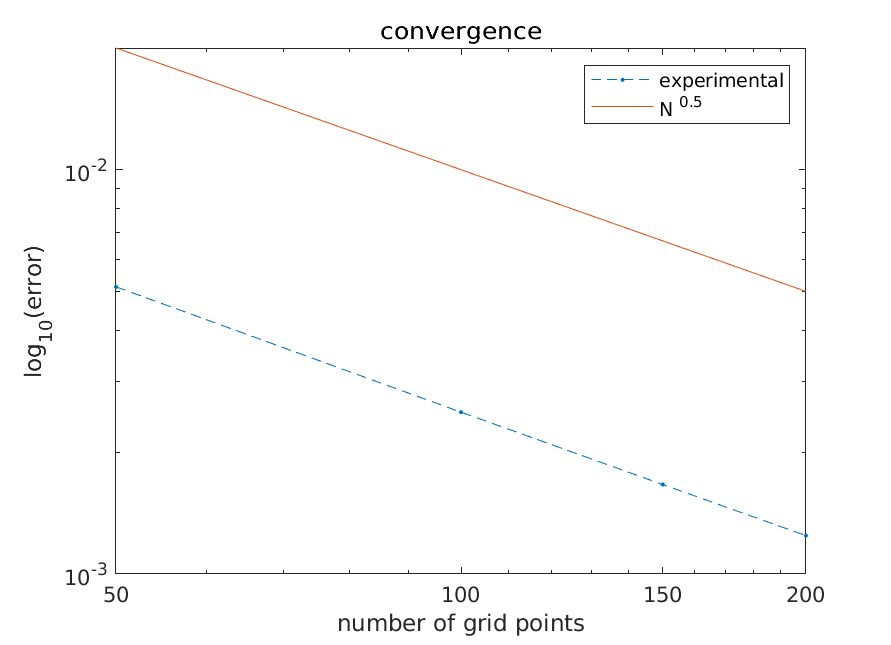
\includegraphics[width=0.55\textwidth]{../../introductory_exercises/diffusion_implicit_1D_solver/data/convergence.png}
\caption{Convergence behaviour for 1D implicit solver (diffusion equation)}
\label{1D_implicit_diffusion}
\end{figure}


\subsubsection{ADI 2D Solver}
\paragraph{Goal} Implement implicit solver for time-dependent diffusion equation
\begin{equation}
\partial_t u(t,x,y) = \partial_{xx}u(t,x,y) + \partial_{yy}u(t,x,y)
\end{equation}
\paragraph{Solution}
There is still an error in the code. 


\subsubsection{Area of a circle}
\paragraph{Goal}
Develop Monte Carlo code
\paragraph{Solution}

\subsection{Other Exercises}
From course material from Ivan Milic.
\subsubsection{Lecture 7}
\begin{enumerate}
\item Derive expressions for the emergent radiation when properties are the following:
\begin{itemize}
\item optically thin slab at all wavelengths
\item wavelength-independent incident radiation
\end{itemize}
Solution: see slide 14?

\item Derive ralations between Einstein coefficients.

\item Calculate electron density in atmosphere from FALC model
\end{enumerate}


\newpage
\section{Limb darkening}
\label{limb_darkening_program_discussion}

\subsection{Formulation of the problem}
\begin{itemize}
\item The radiative transfer equation \ref{GENERAL_RT_EQUATION} in this situtation becomes an integro-differential equation with  $S(\tau) = \frac{1}{4\pi} \int I(\tau,\mu) d\Omega$
\begin{equation}
\begin{aligned}
\mu \frac{dI(\tau,\mu)}{d\tau} &= -I(\tau,\mu) + S(\tau)  \\ 
&= -I(\tau,\mu)  + \frac{1}{4\pi} \int I(\tau,\mu) d\Omega
\end{aligned}
\label{RTE_limb_darkening}
\end{equation}

\item The difficulty resides in the (evaluation of) the source function. Monte Carlo simulation avoids explicit calculation source function: source function implicit in Monte Carlo simulation. There the physics are simulated \textsc{in between two consecutive scattering events} as follows
\begin{equation}
\frac{dI}{dz} = -\alpha I 
\end{equation}
thus $I = I_0 e^{-\delta \tau}$ and then $\tau$ is sampled according to $\tau = - \log(X_{\text{random}})$
\end{itemize}

\subsection{Solving the (integro-differential) radiative transfer equation}
\paragraph{Analytical Solution of Equation (\ref{RTE_limb_darkening})}
Ik heb de mosterd gehaald op \cite{Dublin_limb_darkening}.

\begin{equation}
I(0,\mu) = \int_0^{\infty} S(\tau) exp\left( \frac{-\tau}{\mu} \right) d\left( \frac{\tau}{\mu} \right)
\end{equation}

\paragraph{Numerical Solution of Equation (\ref{RTE_limb_darkening})}
First rewrite the equation
\begin{equation}
\begin{aligned}
\mu \frac{dI(\tau,\mu)}{d\tau} 
&= -I(\tau,\mu)  + \frac{1}{4\pi} \int I(\tau,\mu) \sin(\theta) d\theta d\phi 
\\ &= -I(\tau,\mu)  + \frac{1}{4\pi} \int I(\tau,\mu) d\mu d\phi 
\\ &= -I(\tau,\mu)  + \frac{1}{2} \int I(\tau,\mu) d\mu 
\end{aligned}
\end{equation}
Discretization scheme:
\begin{equation}
???
\end{equation}


\subsection{Eddington-Barbier approximation} 
\begin{equation}
J(\tau) = 3H \left( \tau + \frac{2}{3} \right)
\label{Eddington_Barbier}
\end{equation}
Together with the time-independent radiative transfer equation (\ref{GENERAL_RT_EQUATION}) in a gray (frequency-independent) planar medium gives \begin{equation}
\mu \frac{\partial I(\tau,\mu)}{\partial \tau} = I(\tau,\mu) - 3H\left(\frac{2}{3}+\tau \right)
\label{rad_transfer_eq_limb_darkening}
\end{equation}
The emergent intensity $I(0,\mu)$ is a solution of Equation (\ref{rad_transfer_eq_limb_darkening}). Its solution for $\tau = 0$ equals 
\begin{equation}
I(\tau = 0,\mu) = I_1 \left( \frac{2}{5} + \frac{3 \mu}{5} \right) 
\end{equation}

with $a= \frac{\sigma}{2 \pi}T_{eff}^4$ and $b = \frac{3 \sigma}{4 \pi}T_{eff}^4$

\subsubsection{Validity of the Eddington-Barbier approximation}
\label{validity_eddington}

If we assume Equuation (\ref{Eddington_Barbier}) then $I = I_1(a+b\mu)$ thus $J = \frac{1}{2} \int(\tau,\mu) d\mu = \frac{1}{2} \int_0^1 (a+b\mu)d\mu $

\noindent\fbox{
  \parbox{\textwidth}{
  dat ziet er hier niet goed uit }}

\subsection{2D Case}
We again have $\mu = \cos(\theta)$. The solution of the radiative transfer equation in \underline{plane-parallel syummetry} with frequency-independent absorption and emission, is 
\begin{equation}
I(\mu) = I_1 (0.4 + 0.6\mu)
\end{equation}
In the Monte Carlo code, the photons are sorted according to the direction that they leave the atmosphere.

\paragraph{Goal}
Calculates the angular dependence of photon's emitted from a plane-parallel, grey atmosphere of radial optical depth \texttt{taumax}. The value of \texttt{tau} determines the position of the photon

\paragraph{Variables and Algorithm}
\begin{itemize}
\item \texttt{muarray} contains emergent photons
\item \texttt{na} number of channels
\item \texttt{dmu} = 1/\texttt{na} width of channels
\item \texttt{nphot} number of photons
\item \texttt{taumax} maximum optical depth
\end{itemize}

\begin{algorithm}
\caption{Limb darkening: compute quantitiy of photons}\label{limb_darkening}
\begin{algorithmic}
\State initialization \\
\quad radial optical depth $\tau$ \\
\quad direction $\mu$

\For{all photons} 

\State $\boxed{\tau = \tau_{max}}$
	\While{\texttt{tau} $\geq 0$} 
	
	\State compute scattering angle \texttt{mu}
	\If{tau $\geq$ taumax} $\boxed{mu = sqrt(x)}$ (initial distribution)
	\Else{ $\boxed{mu = 2*x = 1}$} (isotropic scattering)
	\EndIf
	
	\State tau\_i = -log(x2) 
	\State tau = tau - tau\_i*mu	
		
	\EndWhile
	\State \textbf{end while}

	\State now we know that the photon has left the photosphere	
	\State compute the distribution of all angles \texttt{mu} at which the photon left the photosphere
	
\EndFor
\State \textbf{end for}

\State visualisation: 
	\begin{itemize}
	\item plot photon numbers from $\mu d\mu$ against \texttt{mu}
	\item plot specific intensity from $d\mu$ against \texttt{mu} against 
	\end{itemize}


\end{algorithmic}
\end{algorithm}


\begin{figure}[!htp]
\centering
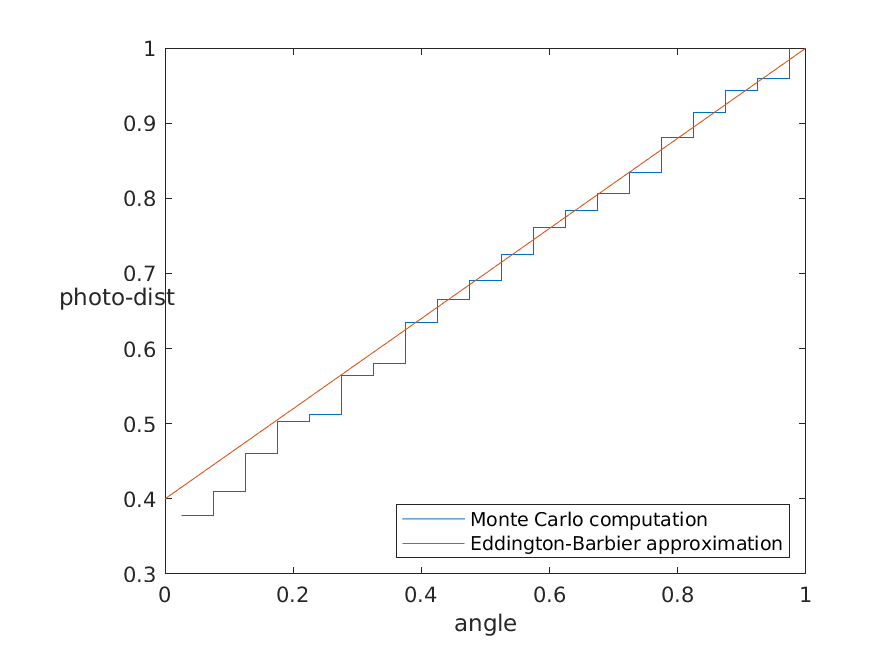
\includegraphics[width=0.7\textwidth]{../../introductory_exercises/limb_darkening/data/number_channels20number_photons100000max_opt_depth10.png}
\caption{histogram for \texttt{mu}}
\label{2D_mu}
\end{figure}
Figure \ref{2D_mu} is according to what is expected $I = I_0(0.4+0.6\mu)$. The input parameters are as follows \texttt{Limb\_Darkening(number\_of\_channels = 20, number\_of\_photons = $10^5$, \\ maximum\_optical\_depth = 10)}.

\newpage
\subsection{3D Case}
\label{3D_limb_darkening}

What changes is this: 
\begin{itemize}
\item introduction of a new angle $\phi$
\item the optical depth is not updated with respect to $\phi$ 
\end{itemize}


\begin{figure}[!htp]
\centering
\begin{minipage}{.5\textwidth}
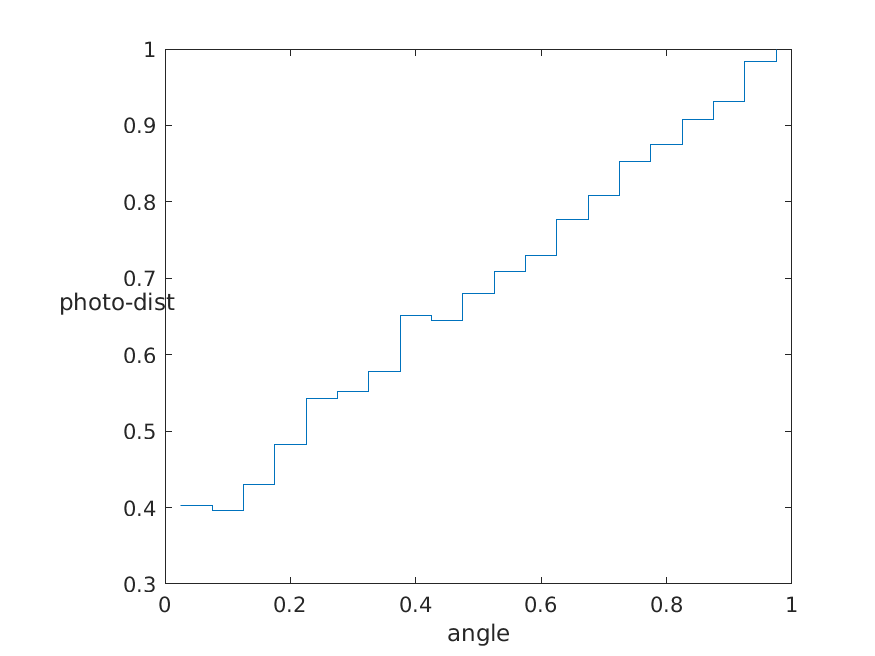
\includegraphics[width=\textwidth]{../../introductory_exercises/limb_darkening/data/LD_3D_mu_number_channels20number_photons100000max_opt_depth10.png}
\caption{histogram for \texttt{mu}}
\label{3D_mu}
\end{minipage}%
\begin{minipage}{.5\textwidth}
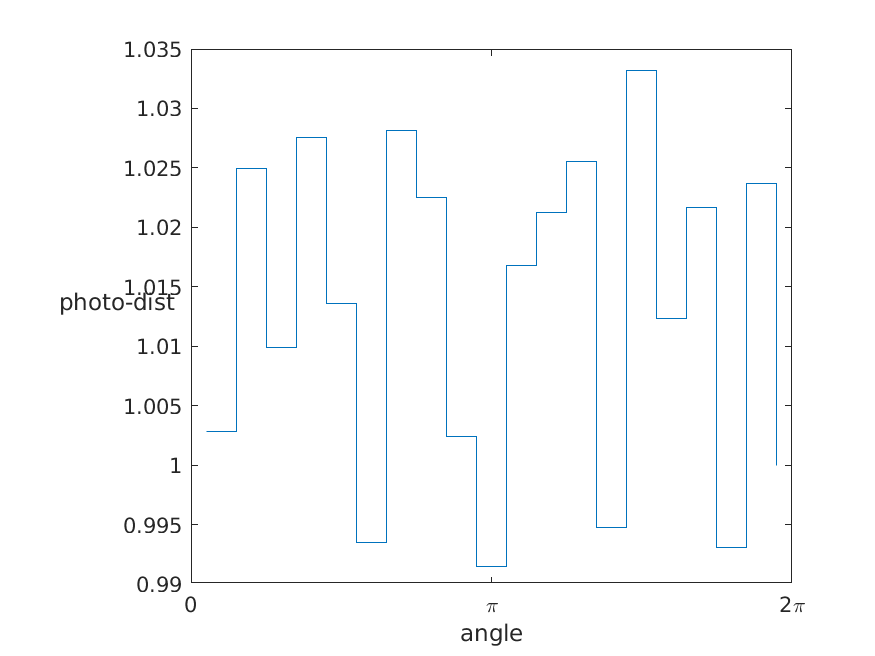
\includegraphics[width=\textwidth]{../../introductory_exercises/limb_darkening/data/LD_3D_phi_number_channels20number_photons100000max_opt_depth10.png}
\caption{histogram for \texttt{phi}}
\label{3D_phi}
\end{minipage}
\end{figure}

Figure \ref{3D_mu} and Figure \ref{3D_phi}  are the result of 
the function \texttt{Limb\_Darkening\_3D} with the following input parameters: \texttt{Limb\_Darkening\_3D(number\_of\_channels = 20, number\_of\_photons = $10^5$, \\ maximum\_optical\_depth = 10)}. The results according to what is expected, namely $I = I_0(0.4+0.6\mu)$ and $\phi$ follows a uniform distribution.

\paragraph{}
\noindent\fbox{
  \parbox{\textwidth}{
\textbf{Extension}: make version where the optical depth is updated with respect to $\phi$ 
}}

\vspace{0.4cm}
Via this link, you can go back to the exercises overview: Section \underline{\ref{Overview_Part_3}}.


\newpage
\section{Spectral line formation: pcyg.f90}
This section is about the study of line formation in an expanding wind.

\subsection*{Background}
\paragraph{Overview of variables}
\begin{center}
\centering
{\tabulinesep=1.5mm
\begin{tabu}{|c|c|c|}
\hline 
name & explanation \\ \hline \hline

\multicolumn{2}{|c|}{\cellcolor{orange} paramaters} \\ \hline
xk0 & \\ \hline
alpha & velocity profile parameter \\ \hline
beta & velocity profile parameter \\ \hline \hline

\multicolumn{2}{|c|}{\cellcolor{orange} start frequency of the photon} \\ \hline
xstart & start frequency \\ \hline
vmin & \\ \hline
vmax  & \\ \hline

\multicolumn{2}{|c|}{\cellcolor{orange}angle of the photon} \\ \hline
xmuestart & start angle \\ \hline
xmuein & incident angle \\ \hline
xmueou & outward angle \\ \hline
\cellcolor{yellow} pstart & impact parameter \\ \hline
xnew & new photon frequency \\ \hline \hline

\multicolumn{2}{|c|}{\cellcolor{orange} optical depth} \\ \hline
tau & optical depth \\ \hline

\multicolumn{2}{|c|}{\cellcolor{orange} number of photons admin} \\ \hline
nphot & number of photons\\ \hline
nin & photons scattered back into core \\ \hline
nout & photons escaped \\ \hline \hline

\multicolumn{2}{|c|}{\cellcolor{orange} functions} \\ \hline
func & velocity profile \\ 
	& distance from center of star $r$ \\ \hline
	
xmueout & outwards (scattered) angle \\ 
& xk0 \\ 
& alpha \\ 
& r \\ 
& v \\ 
& sigma \\ \hline \hline

nchan & amount of bins \\ \hline
\end{tabu}}
\end{center}

\newpage
\begin{center}
\begin{tikzpicture}
[node distance=2.5cm,auto,>=latex']
    \node [int] (a) {\texttt{pcyg.f90}};
    \node (b) [left of=a,node distance=4cm, coordinate] {a};
    \node (c) [right of=a,node distance=4cm, coordinate] {a};
    \path[->] (b) edge node {\texttt{xstart}} (a);
    \path[->] (a) edge node {\texttt{xnew}} (c);
\end{tikzpicture}
\end{center}
The photons are sorted according to \texttt{xnew}.
In general, the flux is dependent on $\mu$ and the frequency $x$.


\paragraph{Practical formula}
\begin{itemize}
\item emission angle $\mu = \cos(\theta)$
\item according p-ray $p = \sqrt{1-\mu^2} = \sin(\theta)$
\item incident angle $\texttt{xmuein} = \sqrt{1-\left(\frac{pstart}{r}\right)^2}$
\end{itemize}

\paragraph{Geometry \& Symmetry assumptions}
\begin{itemize}
\item spherical geometry
\end{itemize}

\subsubsection{Experimental results}
In original version of the code, all photons are released isotropially from the photosphere.

\begin{figure}[!htp]
\centering
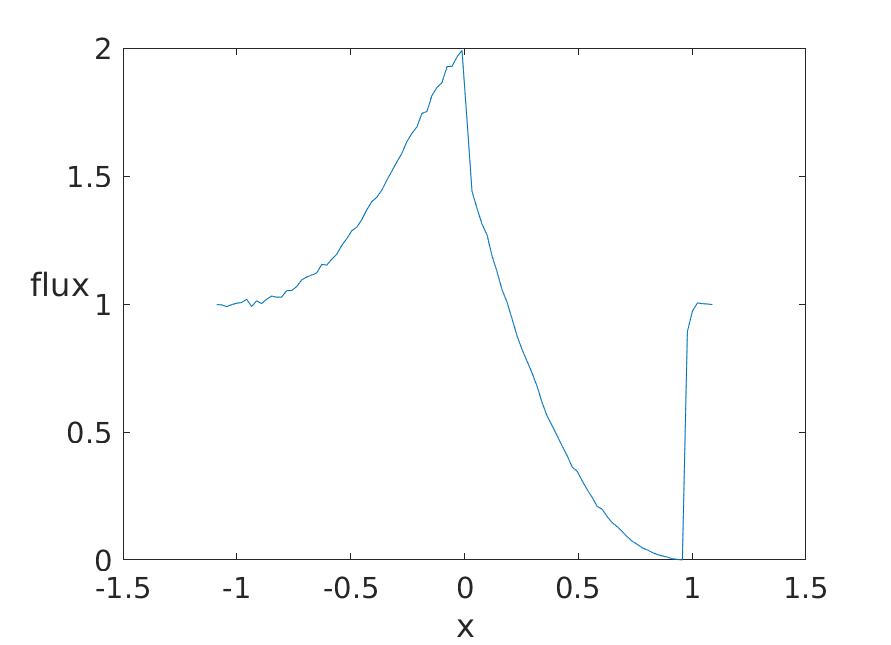
\includegraphics[width=0.5\textwidth]{../../introductory_exercises/P_Cygni_profile_UV_resonance/data/npot6xk0100alpha0beta1test0.png}
\caption{Original version of the code \\ AMOUNT OF PHOTONS?}
\end{figure}

\newpage
\subsection{First adaptation: what if all photons are released radially from photosphere?}
\label{PCYG FIRST adaptation}

\subsubsection{\underline{Release photons radially: numerical MC experiments}}
What would happen with line-profile, if you assumed all photons
were released radially from photopshere?
\begin{itemize}
\item In other words $\texttt{xmuestart} = 1$. 
\item This is implemented under the test case \texttt{test\_number=1}.
\item Results in Figure \ref{PCyg_mu_eq_1} for opacity \texttt{xk0 = 100}.
\end{itemize}

\begin{figure}[!htbp]
\centering
\begin{subfigure}{.5\textwidth}
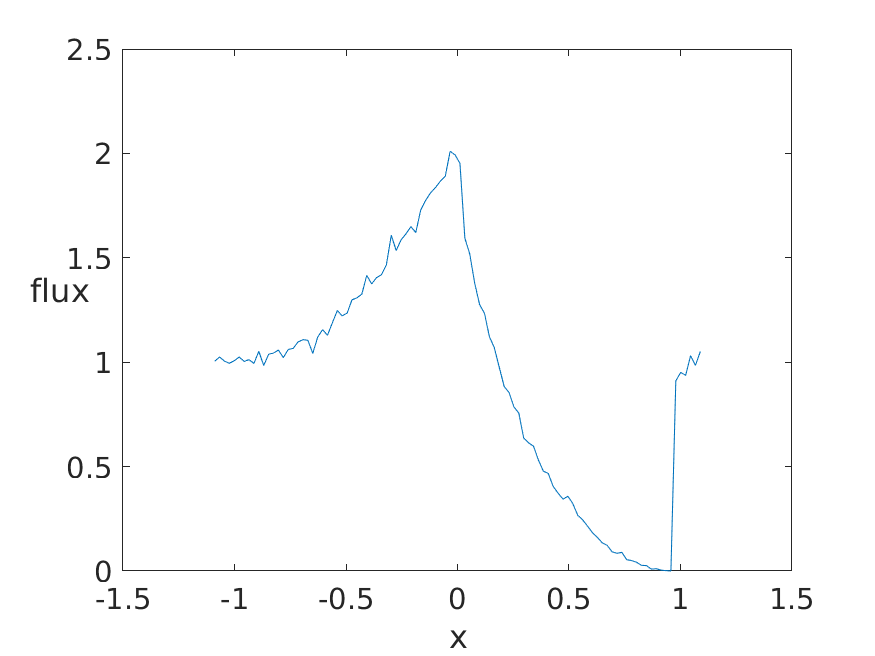
\includegraphics[width=1\textwidth]{../../introductory_exercises/P_Cygni_profile_UV_resonance/data/npot5xk0100alpha0beta1test1.png}
\caption{First adaptation}
\end{subfigure}%
\begin{subfigure}{.5\textwidth}
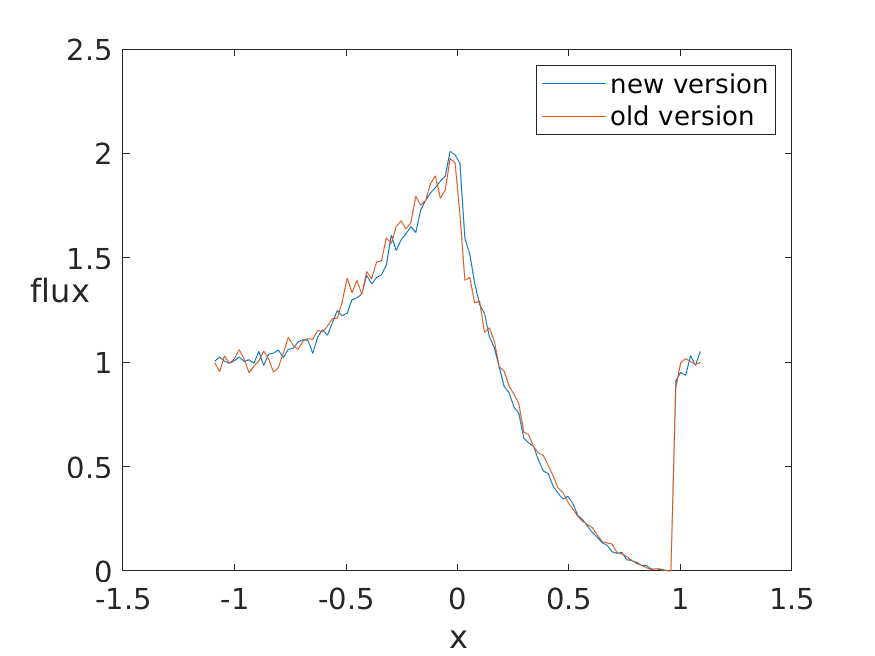
\includegraphics[width=1\textwidth]{../../introductory_exercises/P_Cygni_profile_UV_resonance/data/npot5xk0100alpha0beta1test10.png}
\caption{Same plot (together with output of initial version)}
\end{subfigure}
\caption{The number of photons equals $10^{5}$, \texttt{xk0=100}}
\label{PCyg_mu_eq_1}
\end{figure}


\subsubsection{\underline{Derive analytic expression}} See also slide  26/49 [Sundqvist course material]. 
\begin{itemize}
\item since \texttt{xmuein = 1} we have for the velocity profile 
\begin{equation}
v = v_{\infty}(1-b/r)^{\beta}
\label{velocity_profile}
\end{equation}
A scaled version of Equation (\ref{velocity_profile}) yields 
\begin{equation}
u = \frac{v(r)}{v_{\infty}} = \left(1 - \frac{r_{\infty}}{r} \right)^{\beta} 
\label{u_profile}
\end{equation}
with $u \in [0..1]$

\item Doppler shift for the frequency of the photons: $x_{CMF} = x_{REF} - \mu u$.
\item Condition for resonance from Sobolov approximation (to be studied later): $\boxed{x_{CMF}= 0}$ thus 
\begin{equation}
x_{REF} = \mu u
\label{analytic_profile}
\end{equation}
or thus $x_{REF} = \boxed{u_{\text{interaction}}}$ and than solve Equation \ref{u_profile} for $r_{\text{interaction}}$


\item If $\mu = 1$ then 
\begin{equation}
x = \left(1 - \frac{r_{\infty}}{r} \right)^{\beta}
\end{equation}
\begin{equation*}
x^{1/\beta} = 1 - \frac{r_{\infty}}{r}
\end{equation*}
\begin{equation*}
r(1-x^{1/\beta}) = r_{\infty}
\end{equation*}
\begin{equation}
\boxed{r(x) = \frac{r_{\infty}}{1-x^{1/\beta}}}
\end{equation}

\noindent\fbox{
  \parbox{0.6\textwidth}{
  attention, here was something wrong! }} 

\item From the location of interaction $r$, the incident angle can be calculated
\begin{equation}
\texttt{xmuein} = \sqrt{1-\left[\frac{\texttt{pstart}}{r}\right]^2} = \sqrt{1 - \left[ \frac{\sqrt{1-\texttt{xmuestart}^2}}{r} \right]^2}
\end{equation}
Now also taking into account that \texttt{xmuestart = 1} then yields
\begin{equation}
\texttt{xmuein = 1}
\end{equation}

\item The calculation of the optical depth goes as follows:
\begin{equation}
\tau = \frac{\texttt{xkO}}{rv^{2-\alpha}(1+\texttt{xmuein}^2 \sigma)}
\end{equation}
Now also taking into account that \texttt{xmuestart = 1} gives
\begin{equation}
\tau = \frac{\texttt{xk0}}{rv^2(1+\sigma)}
\end{equation}

where $\boxed{v(x) = \left(1 - \frac{b}{r} \right)^{\beta}}$ 
\quad and $\frac{dv}{dr} = \frac{\beta b}{r^2}\left( 1 - \frac{b}{r} \right)^{\beta - 1}$  \\
and $\sigma(x) = \frac{dv}{dr}\frac{r}{v}-1$ 
thus $\boxed{\sigma(x) = \frac{\beta b}{r}\left( 1-\frac{b}{r}\right)^{-1}}$

\item Assuming that $\beta = 1$ then $\boxed{v(x) = 1 - \frac{b}{r}}$ and $\frac{dv}{dr} = \frac{\beta b}{r^2}$ and $\boxed{\sigma(x) = \frac{\beta b}{r}}$.

\item Conclusion: $\tau(x)$ is only dependent on $x$ and not on \texttt{xmuestart} or \texttt{xmuein}.

\item \texttt{xmueou} follows the distribution as given by the function \texttt{xmueout}, namely
\begin{equation}
p(x) = \frac{1-e^{-\tau}}{\tau}
\end{equation}
with $\tau = \frac{\texttt{tau0}}{1+\texttt{X}^2 \sigma}$ where $\texttt{X}$ is a random number, so actually this comes down to
\begin{equation}
\boxed{p(x) = \frac{1-e^{-\frac{\tau_0}{1+x^2\sigma(x)}}}{\frac{\tau_0}{1+x^ 2\sigma(x)}}}
\end{equation}

\item Finally one can combine these results to get the distribution of the photons according to the frequency $x$ via the relation 
\begin{equation}
\texttt{xnew = xstart + v(xmueou-xmuein) = xstart + v(xmueou -1)}
\label{pcyg_mu_1_final_eq}
\end{equation}

In words, we initially have an isotropic distribution for \texttt{xstart}. The number of photons that are leaving the atmosphere at different frequencies is however not isotropic through complex interactions that are incorporated into $p(x)$.
One must also take into account that not all of the photons that are released actually escape from the atmosphere and also that sometimes no resonance is possible, and then Equation (\ref{pcyg_mu_1_final_eq}) is not applicable.

\end{itemize}

\noindent\fbox{
  \parbox{\textwidth}{TO DO: proceed from this to the analytical expression for the flux. Here I am stuck for the moment.}}
  
\newpage
\subsubsection{\underline{Experiments with other opacities}}
The results for \texttt{xk0=0.5} are shown in Figures \ref{PCyg_mu_eq_1xk0_05} and \ref{PCyg_mu_eq_xk0_05_vs_100}.

\begin{figure}[!htbp]
\centering
\begin{subfigure}{.5\textwidth}
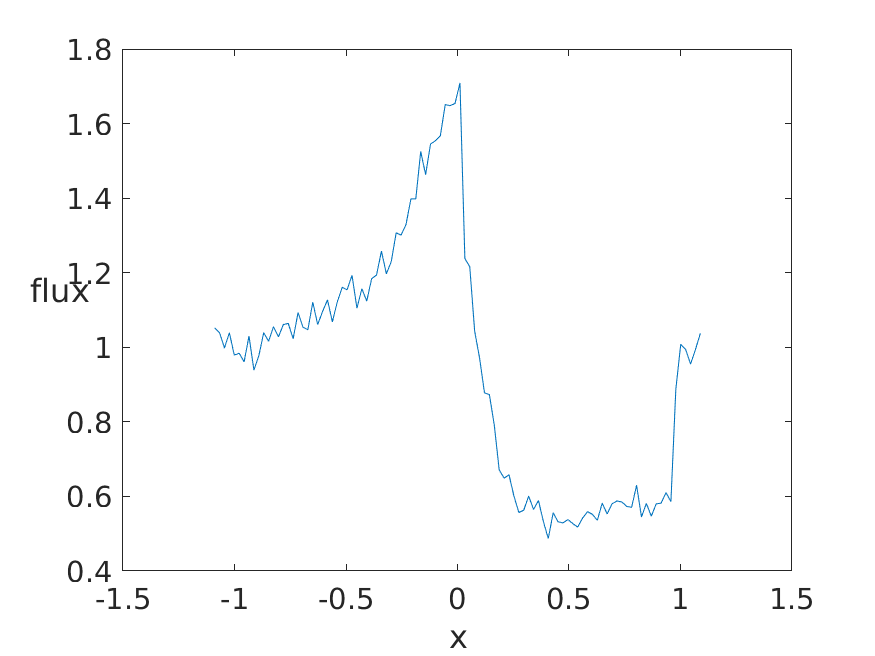
\includegraphics[width=1\textwidth]{../../introductory_exercises/P_Cygni_profile_UV_resonance/data/npot5xk05alpha0beta1test1.png}
\caption{First adaptation}
\end{subfigure}%
\begin{subfigure}{.5\textwidth}
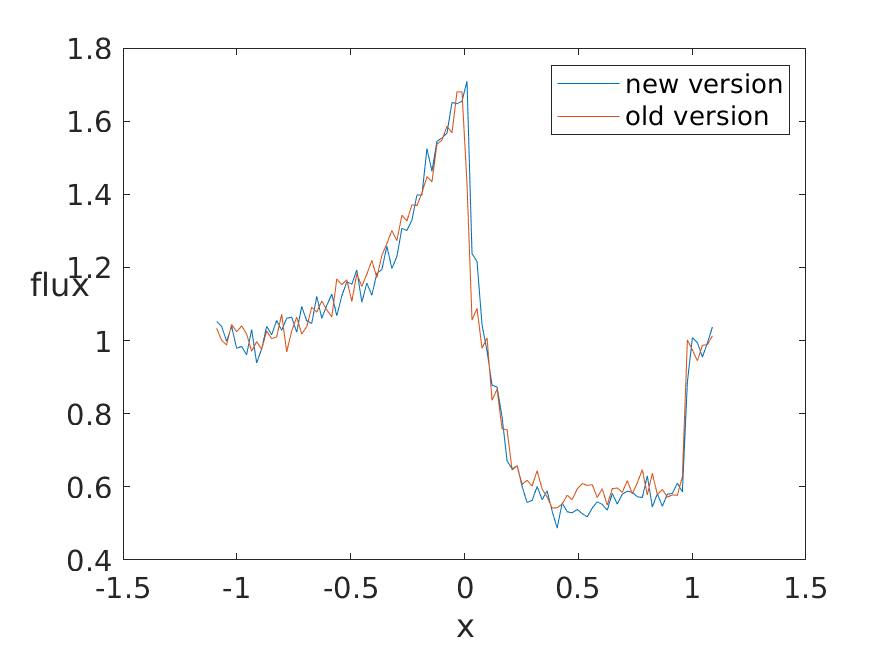
\includegraphics[width=1\textwidth]{../../introductory_exercises/P_Cygni_profile_UV_resonance/data/npot5xk05alpha0beta1test10.png}
\caption{Same plot (together with output of initial version)}
\end{subfigure}
\caption{The number of photons equals $10^{5}$, \texttt{xk0=0.5}}
\label{PCyg_mu_eq_1xk0_05}
\end{figure}

\begin{figure}[!htbp]
\centering
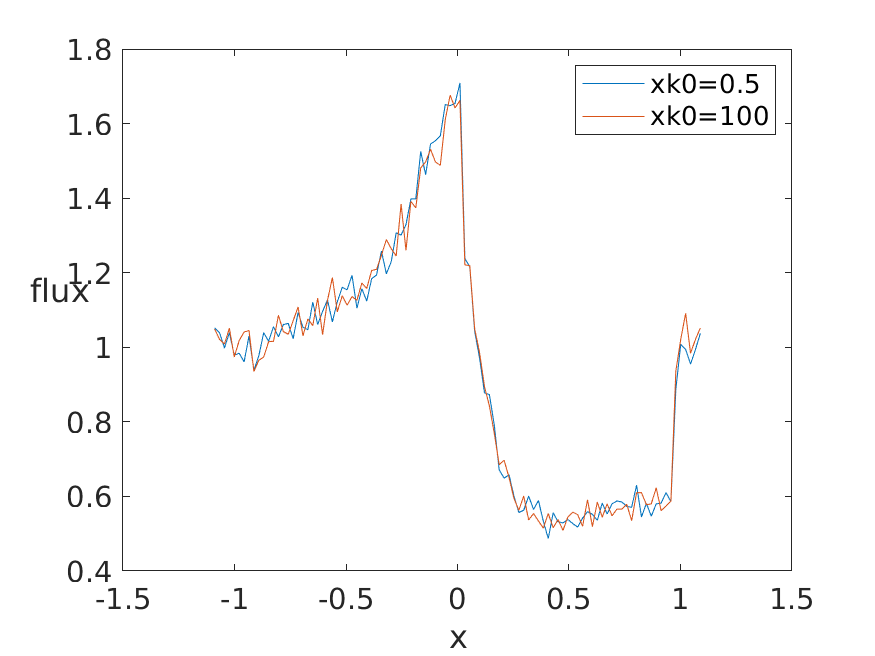
\includegraphics[width=0.5\textwidth]{../../introductory_exercises/P_Cygni_profile_UV_resonance/data/npot5xk05alpha0beta1test11.png}
\caption{The number of photons equals $10^{5}$, \texttt{xk0=0.5}}
\label{PCyg_mu_eq_xk0_05_vs_100}
\end{figure}

Via this link, you can go back to the exercises overview: Section \underline{\ref{Overview_Part_3}}.


\newpage
\subsection{Second adaptation: isotropic scattering}
\label{isotropic_scattering}
What would happen to line-profile, is you assumed scattering
was isotropic 
\\(i.e., NOT following Sobolev-distrobution)

\begin{itemize}
\item in the implementation, \texttt{test\_number = 2}
\item the results are shown in Figure \ref{Pcyg_isotropic_scattering}.
\end{itemize}


\begin{figure}[!htbp]
\centering
\begin{subfigure}{.5\textwidth}
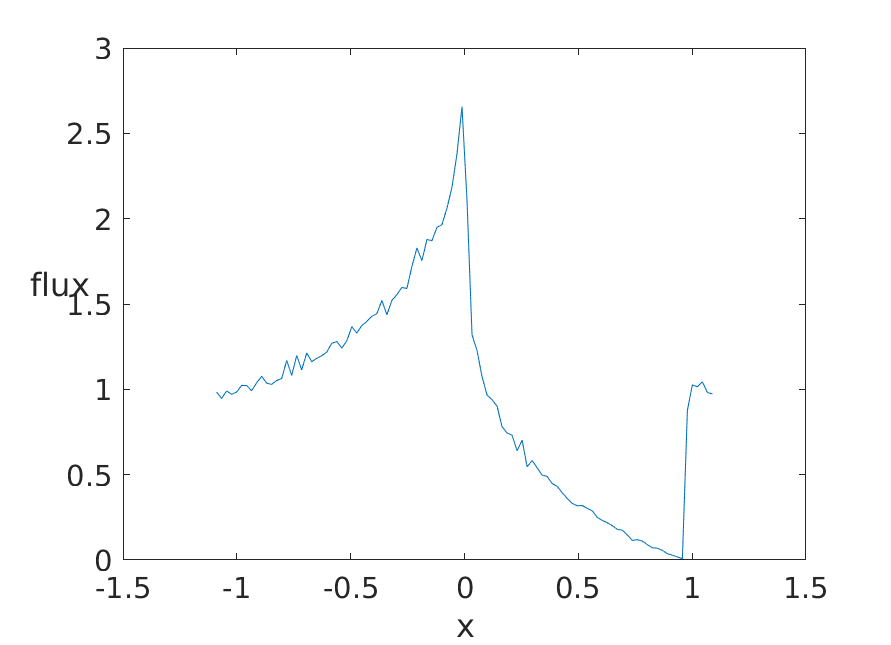
\includegraphics[width=1\textwidth]{../../introductory_exercises/P_Cygni_profile_UV_resonance/data/npot5xk0100alpha0beta1test2.png}
\caption{Second adaptation}
\end{subfigure}%
\begin{subfigure}{.5\textwidth}
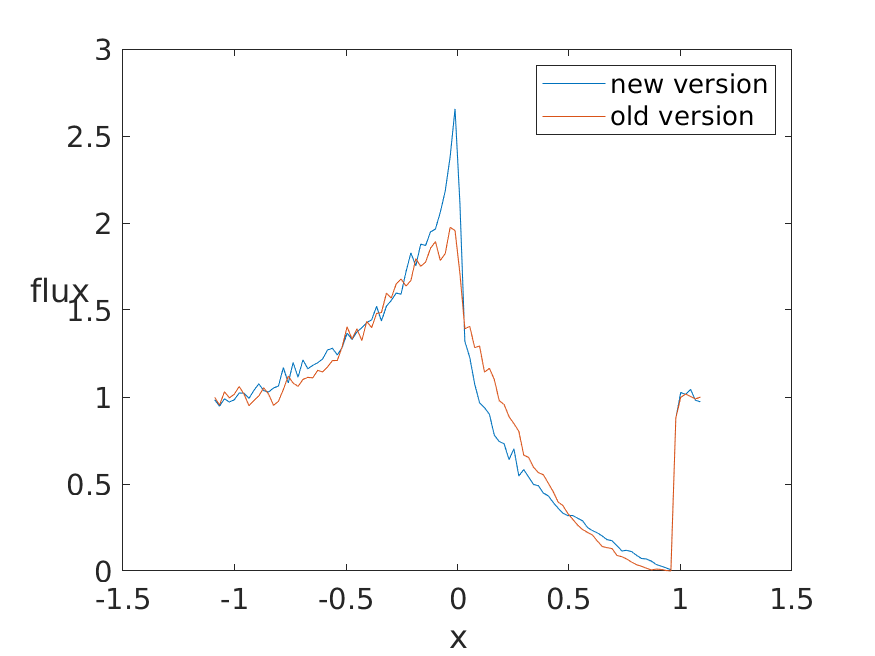
\includegraphics[width=1\textwidth]{../../introductory_exercises/P_Cygni_profile_UV_resonance/data/npot5xk0100alpha0beta1test20.png}
\caption{Same plot (together with output of initial version)}
\end{subfigure}
\caption{The number of photons equals $10^{5}$}
\label{Pcyg_isotropic_scattering}
\end{figure}

It is clear from Figure \ref{Pcyg_isotropic_scattering} that the peak around $x=0$ is higher and sharper. \\
\noindent\fbox{
  \parbox{0.35\textwidth}{Analyse this behaviour more closely}}

\newpage
\subsection{Third adaptation: introduction of Eddington limb-darkening}
\label{Eddington_limb_darkening_adaptation}

\paragraph{Goal} Put Eddington limb-darkening in. What happens? 

\subsubsection{Construction of probability distribution corresponding to Eddington limb darkening}
For a general (introductory) discussion about Eddington limb darkening, please refer to Section \ref{general_limb_darkening}


\begin{enumerate}
\item Let us thus first review the emmission case where \underline{the flux in each direction is isotropic} i.e. $I(\theta) = I$ (as experimented in paragraph \ref{isotropic_scattering})
\begin{itemize}
\item the specific intensity is defined as $I_{\nu}(\mu) = \frac{dE_{\nu}}{\cos(\theta) dA dt d\nu d\Omega} = \frac{dE_{\nu}}{\mu dA dt d\nu d\Omega}$ 
\item the flux $F_{\nu} = \int_{\Omega} I_{\nu} \cos(\theta) d\Omega$ is in this case isotropic thus
\begin{equation}
\xi = \int_0^{\mu} F_{\nu} d\mu = \int_0^{\mu} \int_{\Omega} I_{\nu} \cos(\theta) d\Omega d\mu = A \int_0^{\mu} \mu d\mu   
\end{equation}
together with the condition that $\mu$ satisfies a probability distribution: 
\begin{equation}
1 = \int_{-1}^{1} F_{\nu} d\mu = \int_{-1}^{1} \int_{\Omega} I_{\nu} \cos(\theta) d\Omega d\mu = \frac{A}{2}
\label{isotropic_flux_isotropic_intensity_prob_dist}
\end{equation}
thus $A=2$. Photons need to be sampled according to $\mu d\mu$.
\end{itemize}

\item Now we look at a new case where the photons need to be emitted following a distrubution that corresponds to $I(\theta) = I(0)(0.4+0.6\cos(\theta))$. 
\begin{itemize}
\item in this case the flux $F_{\nu} = \int_{\Omega} I_{\nu} \cos(\theta) d\Omega$ is isotropic but also satisfies
\begin{equation}
F_{\nu} = \int_{\Omega} I_{\nu}(0)[0.4+0.6\cos(\theta)] \cos(\theta) d\Omega
\end{equation} 
\noindent\fbox{
  \parbox{0.8\textwidth}{
I am not sure about the correctness of the assumption of isotropy of the flux}}
\begin{equation}
\xi = \int_0^{\mu} F_{\nu} d\mu = A \int_0^{\mu} (0.4+0.6\mu) \mu d\mu   
\end{equation}
subject to the normalisation condition -very similar to Equation (\ref{isotropic_flux_isotropic_intensity_prob_dist}) - that
\begin{equation}
1 = \int_{0}^{1} F_{\nu} d\mu = \frac{2A}{5}
\end{equation}
thus $A = \frac{5}{2}$. Photons need to be sampled according to
\begin{equation}
\frac{5}{2}(0.4+0.6\mu)\mu d\mu
\label{prob_dist_Eddington}
\end{equation}
\end{itemize}

In the code \texttt{pcyg.f90} this corresponds to \texttt{test\_number = 3} (not yet implemented). 

The results of an accept-reject method that samples the probability distribution in Equation (\ref{prob_dist_Eddington}).

\begin{figure}[!htp]
\centering
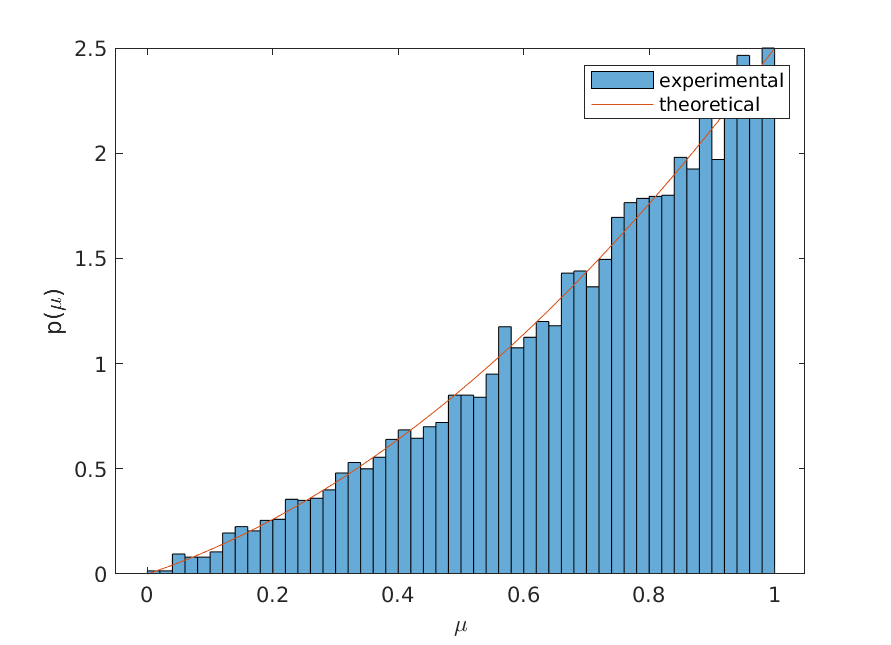
\includegraphics[width=0.55\textwidth]{../../introductory_exercises/P_Cygni_profile_UV_resonance/data/Eddington_accept_reject.png}
\caption{Accept-reject method for Eddington limb darkening}
\end{figure}
\end{enumerate}

Via this link, you can go back to the exercises overview: Section \underline{\ref{Overview_Part_2}}.

\newpage
\subsection{Fourth adaptaion: photospheric line-profile}
Challening: Put photospheric line-profile (simple Gaussian) in. What happens? Test on \texttt{xk0=0} (opacity = 0) case.

\begin{itemize}
\item test case number 4 
\item \noindent\fbox{
  \parbox{0.5\textwidth}{This is still to be implemented.}}
\end{itemize}

\newpage
\subsection{Convergence analysis}
\label{convergence_analysis}

\paragraph{\underline{Zero opacity}}
The convergence of the Monte Carlo method is tested with the following input parameters

\begin{center}
\centering
{\tabulinesep=1.5mm
\begin{tabu}{|c|c|c|c|}
\hline 
\texttt{kx0} & alpha & beta & \texttt{test\_number} \\
0 & 0 & 1 & 0 \\ \hline
\end{tabu}}
\end{center}

for a varying amount of photons, as shown in Figure \ref{Convergence_Pcyg_kx0_0}. We expect the method to have $\frac{1}{\sqrt{N}}$ convergence, where $N$ is the number of photons. However, the methods strangely seems to have a faster convergence rate. 

\begin{figure}[!htp]
\centering
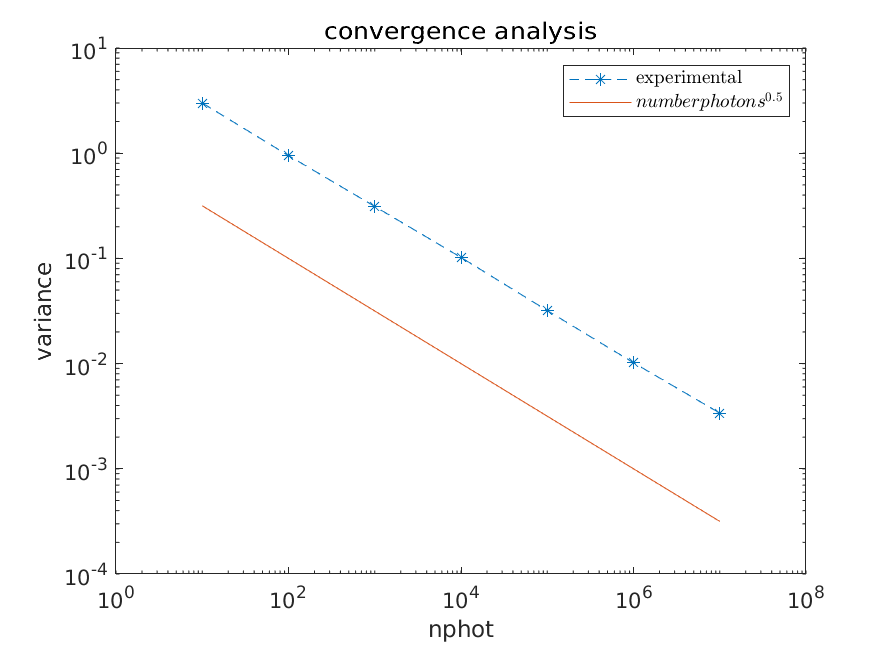
\includegraphics[width=0.5\textwidth]{../../introductory_exercises/P_Cygni_profile_UV_resonance/data/test0_convergence.png}
\caption{Original version of the code: convergence analysis (xk0=0)}
\label{Convergence_Pcyg_kx0_0}
\end{figure}

\paragraph{\underline{Nonzero opacity}} 
The convergence test is set up as follows: different Monte Carlo simulations (with increasing number of photons) are compared to an \textit{expensive} simulation with $10^7$ photons. As can be seen in Figure \ref{Convergence_Pcyg_kx0_100}, the spectrum profile behaves according to a $N^{0.5}$ law.

\begin{figure}[!htp]
\centering
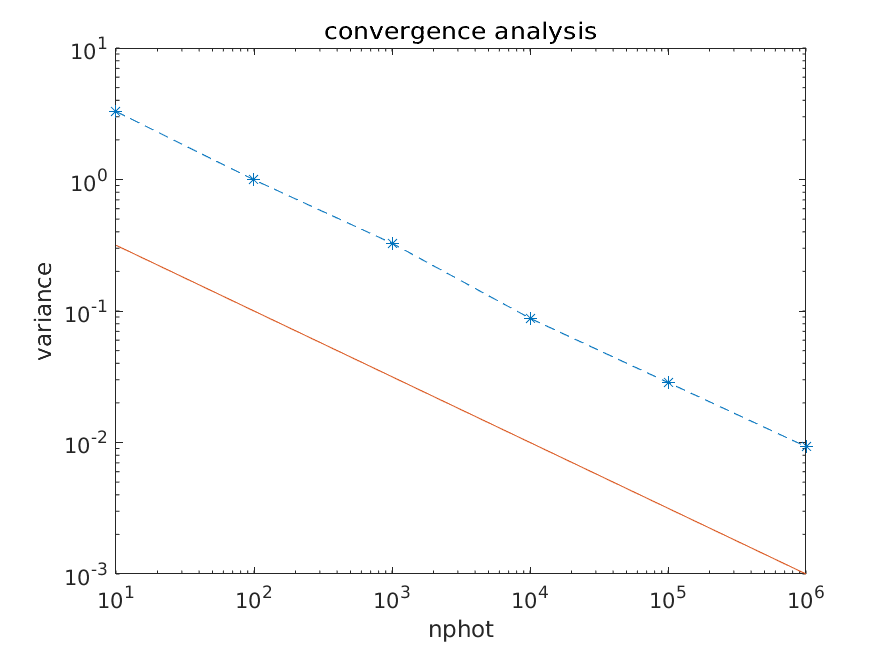
\includegraphics[width=0.5\textwidth]{../../introductory_exercises/P_Cygni_profile_UV_resonance/data/profile_convergence/test0_convergence.png}
\caption{Original version of the code: convergence analysis (xk0=100)}
\label{Convergence_Pcyg_kx0_100}
\end{figure}


Via this link, you can go back to the exercises overview: Section \underline{\ref{Overview_Part_2}}.


\newpage
\subsection{Variance reduction experiment}
\label{variance_reduction_experiment}

We will set up the test as follows
\begin{itemize}
\item run the code with \texttt{xk0=100} and number of photons $N=10^7$
\item run the code again for lower number of photons (e.g. $N=10^3$), both with random sampling and pseudo-random sampling
\item compute variance w.r.t. \textit{expensive} simulation and compare
\item \texttt{test\_number = 5}
\end{itemize}

\paragraph{\texttt{xk0=100}}

\begin{figure}[!htp]
\centering
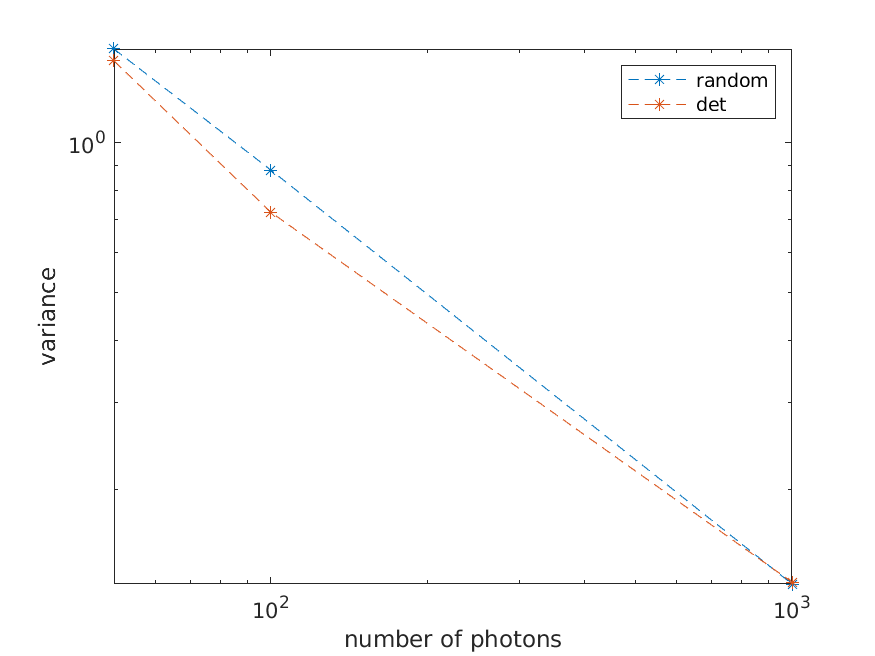
\includegraphics[width=0.65\textwidth]{../../introductory_exercises/P_Cygni_profile_UV_resonance/data/variance_reduction_test.png}
\caption{Original version of the code: convergence analysis (xk0=0)}
\label{variance_reduction_test}
\end{figure}

\noindent\fbox{
  \parbox{0.7\textwidth}{
Possible improvement: average over different stochastic realizations.}}

\vspace{0.7cm}
Via this link, you can go back to the exercises overview: Section \underline{\ref{Overview_Part_3}}.

\subsection{Mathematical description of the problem \&
Looking at literature}
Have a look at \cite{NoebauerUlrichM_2019MCRT} (see Appendix).

\newpage
\section{Dual spectral line formation}
\label{two_resonance_lines}

\subsection{Introduction of second line: theoretical}
\label{second_line}
What happens when you add a line (e.g. \@ $x=0.5=a$)? How would you do that?

\subsubsection{Single line}
\begin{center}
\vspace{-0.45cm}
\begin{algorithm}[!htp]
\caption{\texttt{pcyg.f90: one resonance line}}
\label{pcyg_one_line}
\begin{algorithmic}
\For{all photons} 

\begin{enumerate}
\item Release photon with frequency $x$
\item Check if interaction is uberhaupt possible.
\item Solve for distance (radius $r$) of interaction using Sobolev approximation $x_{CMF} = x_{REL} - \mu v(r)$ with $\boxed{x_{CMF} = 0}$ and compute Sobolev optical depth
\item Check whether the photon is scattered:
\end{enumerate}
\If{$\tau_S > -log(\xi)$}
\State Interaction: the photon is scattered. Update the frequency
\Else \State No interaction
\EndIf

\begin{enumerate}
\setcounter{enumi}{3}
\item update the frequency according to the scattering event
\end{enumerate}
	
\EndFor
\State \textbf{end for}
\State collect photons and perform visualisation

\end{algorithmic}
\end{algorithm}
\end{center}

\subsubsection{Introduction of second line}

\noindent\fbox{
  \parbox{0.7\textwidth}{
Needs to be updated}}

\begin{comment}
\begin{center}
\vspace{-0.45cm}
\begin{algorithm}[!htp]
\caption{\texttt{pcyg.f90: introduction of second resonance line}}
\label{pcyg_one_line}
\begin{algorithmic}
\For{all photons} 

\begin{enumerate}
\item Release photon with frequency $x$
\item Check if interaction is uberhaupt possible.
\item Solve for distance (radius $r$) of interaction using Sobolev approximation $x_{CMF} = x_{REL} - \mu v(r)$ with $\boxed{x_{CMF} = 0}$ and compute Sobolev optical depth 
\item \textcolor{blue}{solve $x_{REF} = x_{CMF} - \mu v(r)$ with $\boxed{x_{CMF} = a}$ for $r_{\text{interaction}}$}
\item \textcolor{blue}{Choose the event corresponding with the lowest value of $r_{\text{interaction}}$}
\item Check whether the photon is scattered:
\end{enumerate}
\If{$\tau_S > -log(\xi)$}
\State Interaction: the photon is scattered. Update the frequency.
\textcolor{blue}{Is there a second scattering event?
\begin{enumerate}[leftmargin=0.6in]
\item Check if interaction is uberhaupt possible.
\item Solve $x_{REF} = x_{CMF} - \mu v(r+ r_{\text{interaction}})$ with $\boxed{x_{CMF} =b}$ where $b$ is the frequency where no scattering has yet found place
\item Check whether the photon is scattered:
\end{enumerate}}
\If{\textcolor{blue}{$\tau_{S,2} > -log(\xi_2)$}}
\State \textcolor{blue}{Second interaction: the photon is scattered once again. Update the frequency.}
\Else \State \textcolor{blue}{No second interaction}
\EndIf

\Else \State no interaction
\EndIf	
\EndFor
\State \textbf{end for}
\State collect photons and perform visualisation
\end{algorithmic}
\end{algorithm}
\end{center}

\newpage
pitfalls yet to solve:
\begin{itemize}
\item root must be bracketed
\end{itemize}
\end{comment}

\subsubsection{Algorithm}
\begin{enumerate}
\item release photon
\item $x_{CMF} = x_{REL} - mu v$
\item scattering
\item interaction?
\item scattering
\item collect photons
\end{enumerate}

\paragraph{Ranges and limits}
Assuming $\mu_{start} = 1$. Note that in the code $r_{\infty} = b$

\subsection{Development of computer code}
\subsubsection{Implementation in Matlab: user's manual}
Run the function \texttt{test\_function(test\_number)}.
\begin{center}
\centering
{\tabulinesep=1.5mm
\begin{tabu}{|c|c|c|}
\hline
\texttt{test\_number} & parameter settings \\ \hline \hline
0 & original version \\ \hline
1 & first adaptation: radial release \\ \hline
2 & isotropic scattering -- higher peak \\ \hline
3 & Eddington limb darkening \\ \hline
4 & photospheric line-profile  \\ \hline \hline

5 & simple well \\ \hline
6 & other resonance frequency (thus introducing shift) \\ \hline 
7 & formation of two lines, only radially streaming photons (thus also radial release \\ \hline
8 & formation of two lines, with radial release \\ \hline
9 & formation of two lines, full scattering possibilities \\ \hline
\end{tabu}}
\end{center}


\vspace{0.7cm}
Via this link, you can go back to the exercises overview: Section \underline{\ref{Overview_Part_4}}.

\subsubsection{Keeping track of the photon path}
\begin{equation}
\left[
\begin{matrix}
\texttt{xstart} \\
\texttt{xmuestart} \\
\texttt{r\_new} \\
\hdots \\
\texttt{xmueou} \\
\end{matrix}
\right]
\end{equation}

\subsubsection{Dirty tricks}
\begin{itemize}
\item when \texttt{xnew > xmax} then set \texttt{xnew} to \texttt{xmax}.
\end{itemize}

\newpage
\section{Closer look at Monte Carlo simulations}
\label{diffusion_Monte_Carlo_mean_free_path}

\subsection{Random walk (diffusion equation)} A more simple experiment that simulates the diffusion equation (1D random walk) is also set up. The results are shown in Figure \ref{random_walk_N_vs_tau}.
	\begin{figure}[!htp]
	\centering
	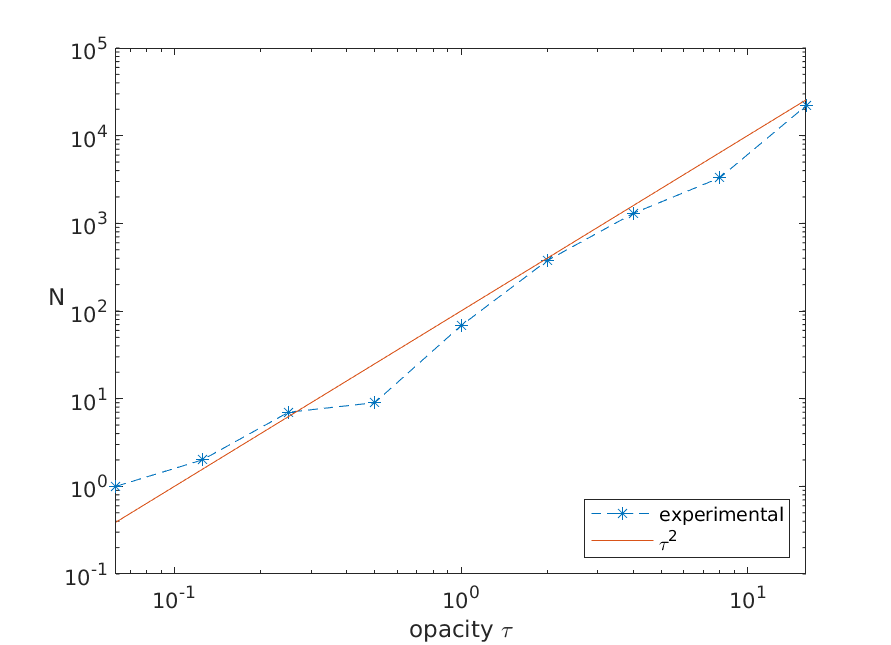
\includegraphics[width=0.5\textwidth]{../../introductory_exercises/limb_darkening/data/diff_N_vs_opacity.png}
	\caption{Number of interactions (scattering events) versus 	opacity, random walk}
	\label{random_walk_N_vs_tau}
	\end{figure}
We observe that $N \sim \tau^2$, as can also be derived from theory.

\begin{itemize}
\item When starting from an initial condition $x_0 = 0$ and 
\begin{equation}
x_N = x_{N-1} \pm l
\end{equation}
we have for the variance that $\braket{x_N}^2 = N l^2$ 
\item If we require a photon to cover a distance $R$ then $N = \frac{R^2}{l^2}$ and
\begin{itemize}
\item the relation between mean-free path $l$ and opacity $\alpha$ is $l = \frac{1}{\alpha}$
\item with $\tau = \int_0^R \alpha ds = \frac{R}{l}$
\end{itemize}
then we have that $N = \tau^2$. This corresponds with the observations in Figure \ref{random_walk_N_vs_tau}.
\end{itemize}

\newpage
\subsection{Iets}

\newpage
\subsection{Limb darkening} We first look at results from the limb darkening program, as studied in Section \ref{limb_darkening_program_discussion}. In Figure \ref{limb_darkening_N_vs_tau}, the number of scattering events is plotted versus the opacity of the medium. 

	\begin{figure}[!htp]
	\centering
	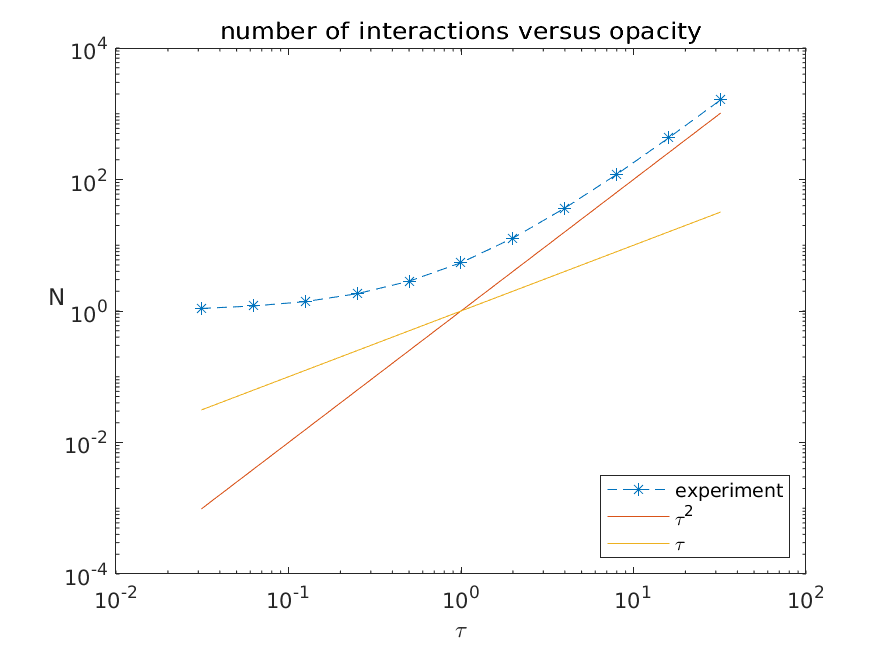
\includegraphics[width=0.5\textwidth]{../../introductory_exercises/limb_darkening/data/N_vs_opacity.png}
	\caption{Number of interactions (scattering events) versus 	opacity, kimb darkening}
	\label{limb_darkening_N_vs_tau}
	\end{figure}

\begin{itemize}
\item For high opacity $\tau \gg 1$ we observe that $N \sim \tau$. \item Bridging regime.
\item For opacity $\tau \ll 1$ we observe that $N \sim 1$: namely the photons travels very far during the first emission event.
\end{itemize}

The splitting scheme from \cite{Dimarco2018} can perfectly be applied to the used Monte Carlo code.


\noindent\fbox{
  \parbox{\textwidth}{
  If you assume constant opacity then $\tau = \alpha z$
  }}

\end{document}
